\newpage
\section{A1.2) Rosetta 2}

\subsection{A.1.2.a)}

\begin{itemize}
    \item \emph{Use T-diagrams to show how Rosetta 2 can execute x86 programs on
      ARM.}
\end{itemize}


\begin{figure}[h]
\centering
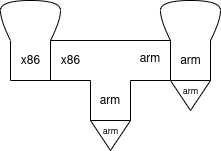
\includegraphics[width=6cm]{../rosetta_2.png}
  \caption{{\scriptsize T-diagram of how Rosetta 2 can execute x86 programs on
  ARM machines.}}
\label{fig:rosetta_2}
\end{figure}

\sectend

\subsection{A.1.2.b)}

\begin{itemize}
    \item \emph{Discuss advantages and disadvantages of this approach over
      recompiling source code to run on ARM.}
\end{itemize}


\paragraph{Advantages}~\smallskip

The main advantage is of course portability. With Rosetta 2, users can run
programs written for x86 on their ARM machines. This means that users can
purchase a new Mac machine without having to let go of their old software
written for x86.

\medskip

This is of course also a huge benefit for the developers, since they do not have
to target two different architectures when they want their software to run on
both new and older machines, but instead simply target x86 and then let users
with newer machines run through Rosetta.

\paragraph{Disadvantages}~\smallskip

the JIT compiler is prone to making bad decisions. It might AOT-compile code
which is not run sufficiently many times to amortize the cost of compilation, or
it might neglect to AOT-compile parts of the code which \emph{is} in fact run
often, potentially producing a bottleneck where there shouldn't be one.

\medskip

In addition, there is some memory overhead in the JIT-compiler, since to
function it essentially needs to keep the interpreter running, whilst
occasionally invoking the compiler. This overhead can be significant if the input
program is small.

\Sectend
